\subsection{Application on the Graph Coloring Game}

\begin{flushleft}

    ......\\~\\

    \subsubsection{Defining Styles of Play}

    \begin{flushleft}

        The process of transforming the underlying dynamic graph-coloring game into its empirical form begins by understanding the different ways in which agents respond in the game. This involves two essential steps:
        %
        \begin{enumerate}
            \item Identifying agents' strategies.
            \item Constructing the empirical game payoff matrix.\\~\\
        \end{enumerate}
        %

        Agents' strategies in the game can be thought of as different styles of play, which are typically revealed through their preferences and behaviors in response to the game’s structure. In our experiments, we specify different styles across three main dimensions: color tone (preference for which colors to use), block difficulty (preference for the types of blocks to choose), and coloring approach (preference for the number of colors to use), as shown in Table~\ref{tab:preferences}. These dimensions are combined to define a player's overall style, which can range from complete indifference—where no specific preference is observed in any of the dimensions (denoted by "I")—to highly specific preferences across all dimensions.\\~\\
        %
        \begin{table}[H]
            \centering
            \begin{tabular}{ll}
                \toprule
                \textit{Preference Dimension} & \textit{Value} \\ 
                \midrule
                Color Tone & warm (W) vs. cool (C) \\ 
                Block Coloring Difficulty & small (L) vs. large (A) \\ 
                Coloring Approach & minimalistic (M) vs. extravagant (E) \\ 
                \bottomrule
            \end{tabular}
            \vspace{0.5em}
            \caption{Dimensions specifying agents' strategies}
            \label{tab:preferences}
        \end{table}
        %
       
        In our approach, policies corresponding to specific strategies are represented using convolutional neural networks (CNNs), which are trained to adapt to different styles of play in the graph-coloring game. To guide the training of these policies, we assign specific values to each of the three dimensions of the game's \emph{preference reward}—color tone, block difficulty, and coloring approach. These values, range from -1 to 1, where 1 indicates a strong preference for a particular dimension. For example, a value of 0.7 for warm colors suggests a relatively strong preference for warm tones, while values closer to 0 a tendency towards indifference. In our experimental setting, we define a total of 11 distinct styles of play: I, C, W, E, M, L, A, AE, CA, LE and WL, given ``I'' and combinations of preference values specified in Table~\ref{tab:preferences}. Assuming no inherent bias among the players of the empirical game, we allow populations to sample from the same list of strategies.

    \end{flushleft}

    \subsubsection{Realizing the Empiricl Game Strategies}

    \begin{flushleft}

        All the policy models used to realize the empirical game strategies share a common underlying architecture and training setup. Although hyperparameter tuning is typically recommended, it doesn't make much difference in this case, as these models are relatively easy to optimize when trained in small settings. Regarding the convolutional neural network architecture, it consists of four convolutional layers, each defined with a kernel size of 3, stride of 1, and padding of 1. These parameters are chosen to ensure that the model is capable of extracting spatial features from the input data, which in this case is a grid representation of the game state. The input tensor has dimensions $10 \times 12$, where $|B|=10$ represents the number of blocks in the state and $|CR^*|=12$ represents the number of possible colors a block can have. Each block is encoded using one-hot encoding, meaning that each color is represented as a binary vector of length 12. The output is then flattened and passed through two fully connected layers, which process the data to produce the final output, as shown in Figure~\ref{fig:convDQN}.\\~\\
        %
        \begin{figure}[H]
            \centering
            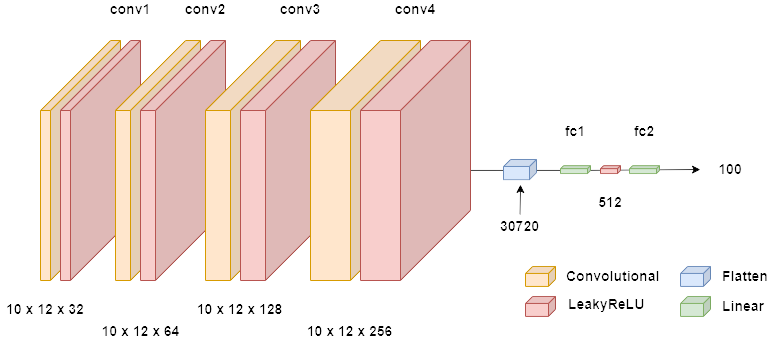
\includegraphics[width=0.8\linewidth]{images/convDQN.png}
            \caption{Convolution Policy Network Architecture}
            \label{fig:convDQN}
        \end{figure}
        %

        Policy models are trained independently in the underlying game using the deep Q-learning reinforcement learning algorithm specified in Algorithm~\ref{alg:dqn_algorithm}. We set $\gamma$ to 0.7. To optimize the model parameters, we use the smooth L1 loss function with $\beta$=1.0 and the Adam optimizer with a learning rate of 5e-4 and weight decay of 1e-5 to prevent over-fitting. To further enhance the learning process, we incorporate experience replay, with a memory that stores up to 10 million experiences \cite{10.1007/BF00992699}. A target network alongside the main policy network, is being used according to the Double-DQN approach \cite{vanhasselt2015deep}. To update the target network we apply a soft update with a factor $\tau$=5e-3. This gradually brings the target network closer to the policy network, balancing learning speed and stability. With a batch size of 64, we train the models for 10,000 episodes.\\~\\
        %
        \begin{algorithm}
            \caption{Double Deep Q-Learning with Experience Replay}
            \label{alg:dqn_algorithm}
            \begin{algorithmic}[1]
            \State $Q_\theta$, $Q_{\theta'} \gets Q_\theta$, $M$ \Comment{Initialize policy/target nets \& memory}
            \For{episode}
                \State $s \gets s_{0}$
                \For{step}
                    \State $a \gets \text{argmax}_a Q_\theta(s)$ \Comment{Select $\epsilon$-greedy action}
                    \State $(s, a, r, s') \in M$ \Comment{Store experience}
                    \If{$|M| > \text{batch size}$} 
                        \For{each $(s, a, r, s')$ in $M$} \Comment{Sample memory}
                            \State $y \gets r + \gamma \max_{a'} Q_{\theta'}(s')$
                            \State $L \gets \text{Loss}(Q_\theta(s), y)$
                            \State $\theta \gets \theta - \alpha \nabla_\theta L$
                        \EndFor
                    \EndIf
                    \State $Q_{\theta'} \gets \tau Q_\theta + (1 - \tau) Q_{\theta'}$ \Comment{Soft update}
                    \State $s \gets s'$
                \EndFor
            \EndFor
            \end{algorithmic}
        \end{algorithm}
        %
        
        In this setup, the agents are trained without any co-players, meaning that each model learns in isolation. This approach is intentional, as our goal is to develop agents that play optimally on their own, rather than in collaboration with others. The idea is to explore how different styles of independent players interact with each other. We expect that some styles will lead to more conflicts than others, and this behavior is key to our analysis. If we had trained the agents together, for example using a multi-agent reinforcement learning (MARL) approach designed for collaborative settings, the resulting agents would have learned joint policies, which would defeat the very purpose of evaluating how their individual  policies affect collaboration.\\~\\

        Let us consider, for instance, the simulation statistics of two relatively compatible play styles that we expect to perform well together in the game: Player W (a human player with preferences for warm color tones) and Player C (a robot with preferences for cool color tones). In Figure~\ref{fig:cw-solution}, we observe how these players' individual preferences shape their interactions. The statistics in Figure~\ref{fig:cw-stats} reveal the most frequently selected actions in terms of blocks and colors. Player C prefers colors like blue, purple, and green, while Player W tends to choose colors like brown, orange, and red. Given these preferences, conflicts are unlikely to arise from color selection alone. Even in scenarios where they may choose to color neighboring blocks, it is highly impossible that both players will choose the same color.\\~\\
        %
        \begin{figure}[H]
            \centering
            \begin{subfigure}[b]{0.45\textwidth}
                \centering
                \raisebox{0.8cm}[0pt][0pt]{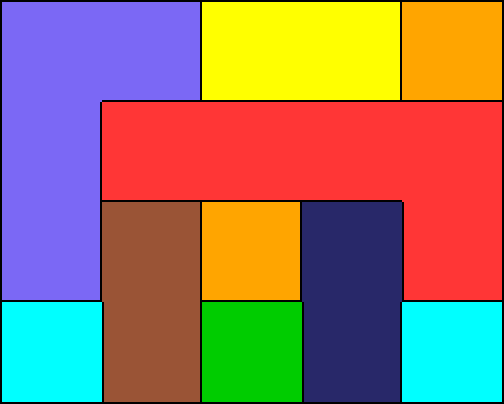
\includegraphics[width=\textwidth]{images/cw-solution.png}}
                \caption{}
                \label{fig:cw-solution}
            \end{subfigure}
            \hspace{0.05\textwidth}
            \begin{subfigure}[b]{0.45\textwidth}
                \centering
                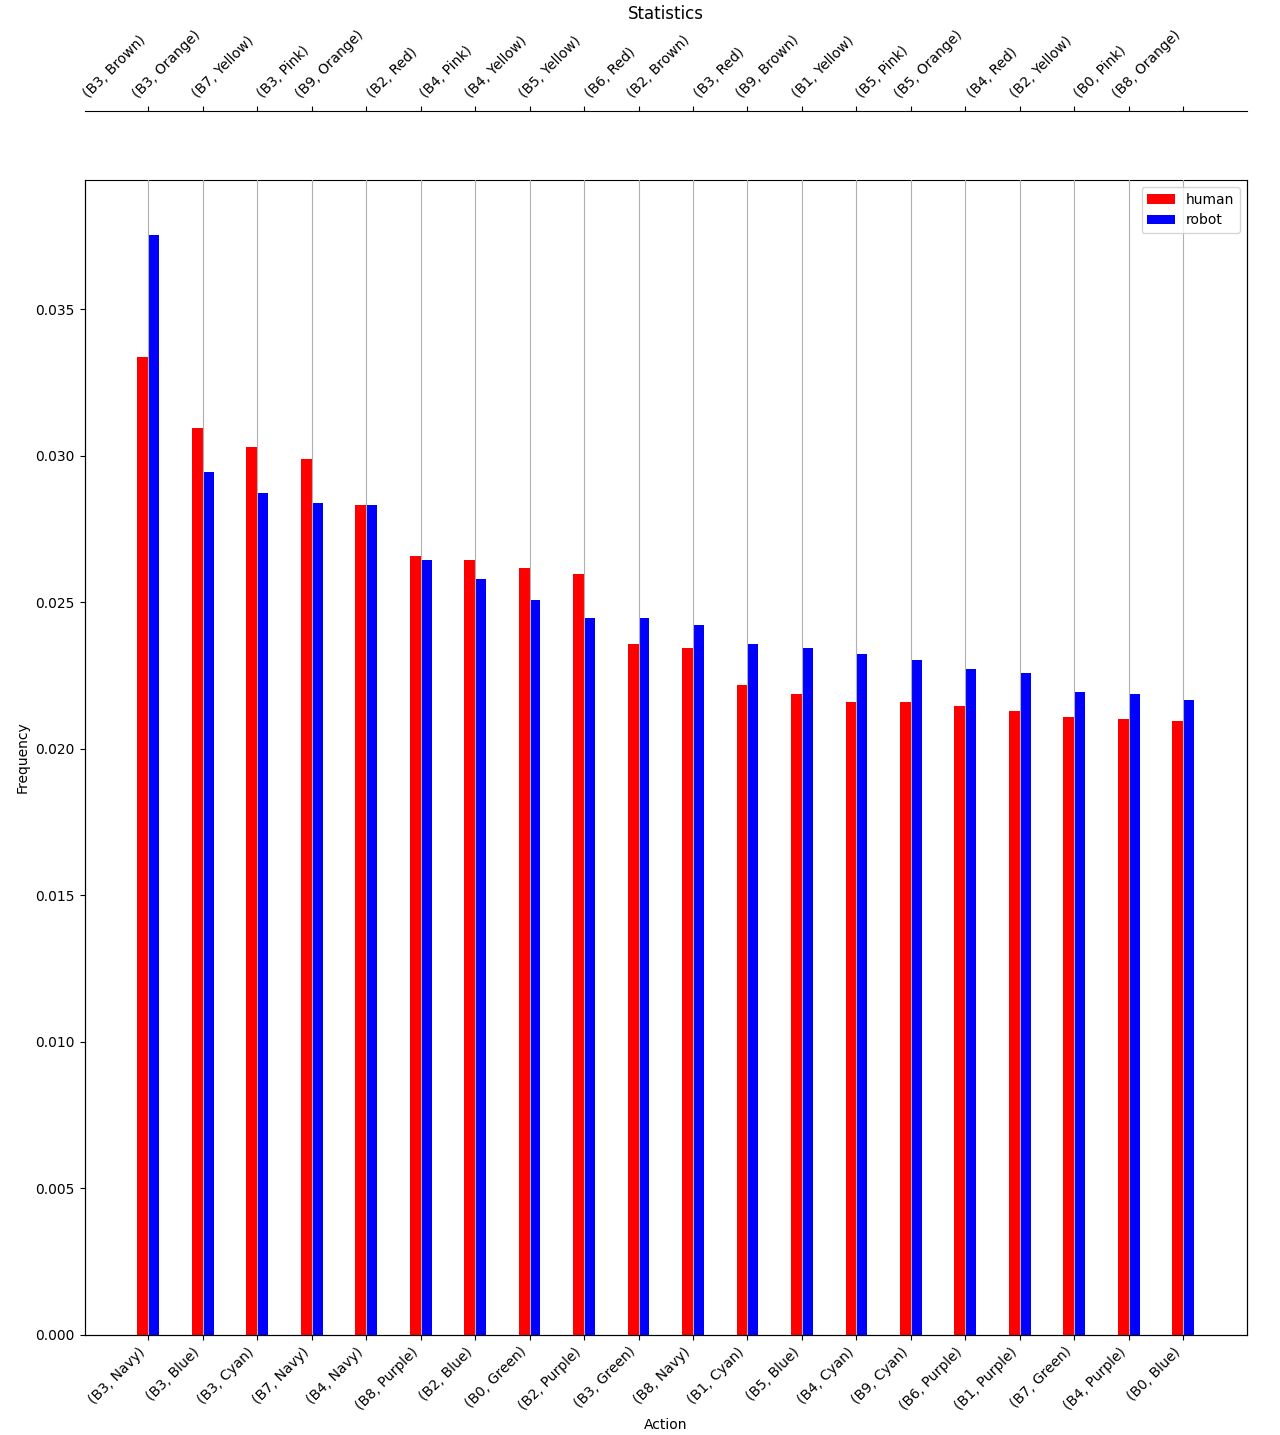
\includegraphics[width=\textwidth]{images/cw-stats.png}
                \caption{}
                \label{fig:cw-stats}
            \end{subfigure}
            \caption{Results from simulating the interactions between players C and W. The left image shows an example solution to the game (a), and the right image presents a statistical analysis of the most frequently selected actions (b).}
            \label{fig:cw-simulation}
        \end{figure}
        %        

        On the other hand, in Figure~\ref{fig:cc-solution}, we observe the interactions between two Player C agents. In this case, we expect more conflicts, as both players share similar color preferences. This increases the likelihood of both players selecting the same color for neighboring blocks. The statistics shown in in Figure~\ref{fig:cc-stats} further support this, as they reveal a high probability of color overlap, primarily due to the dominance of cool colors in both action spaces. However, these conflicts are not a result of insufficient training, but rather stem from the inherent similarity in their preferences.\\~\\
        %
        \begin{figure}[H]
            \centering
            \begin{subfigure}[b]{0.45\textwidth}
                \centering
                \vspace{0.5em}
                \raisebox{0.8cm}[0pt][0pt]{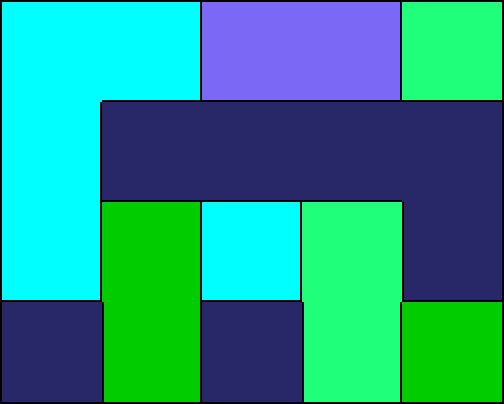
\includegraphics[width=\textwidth]{images/cc-solution.png}}
                \caption{}
                \label{fig:cc-solution}
            \end{subfigure}
            \hspace{0.05\textwidth}
            \begin{subfigure}[b]{0.45\textwidth}
                \centering
                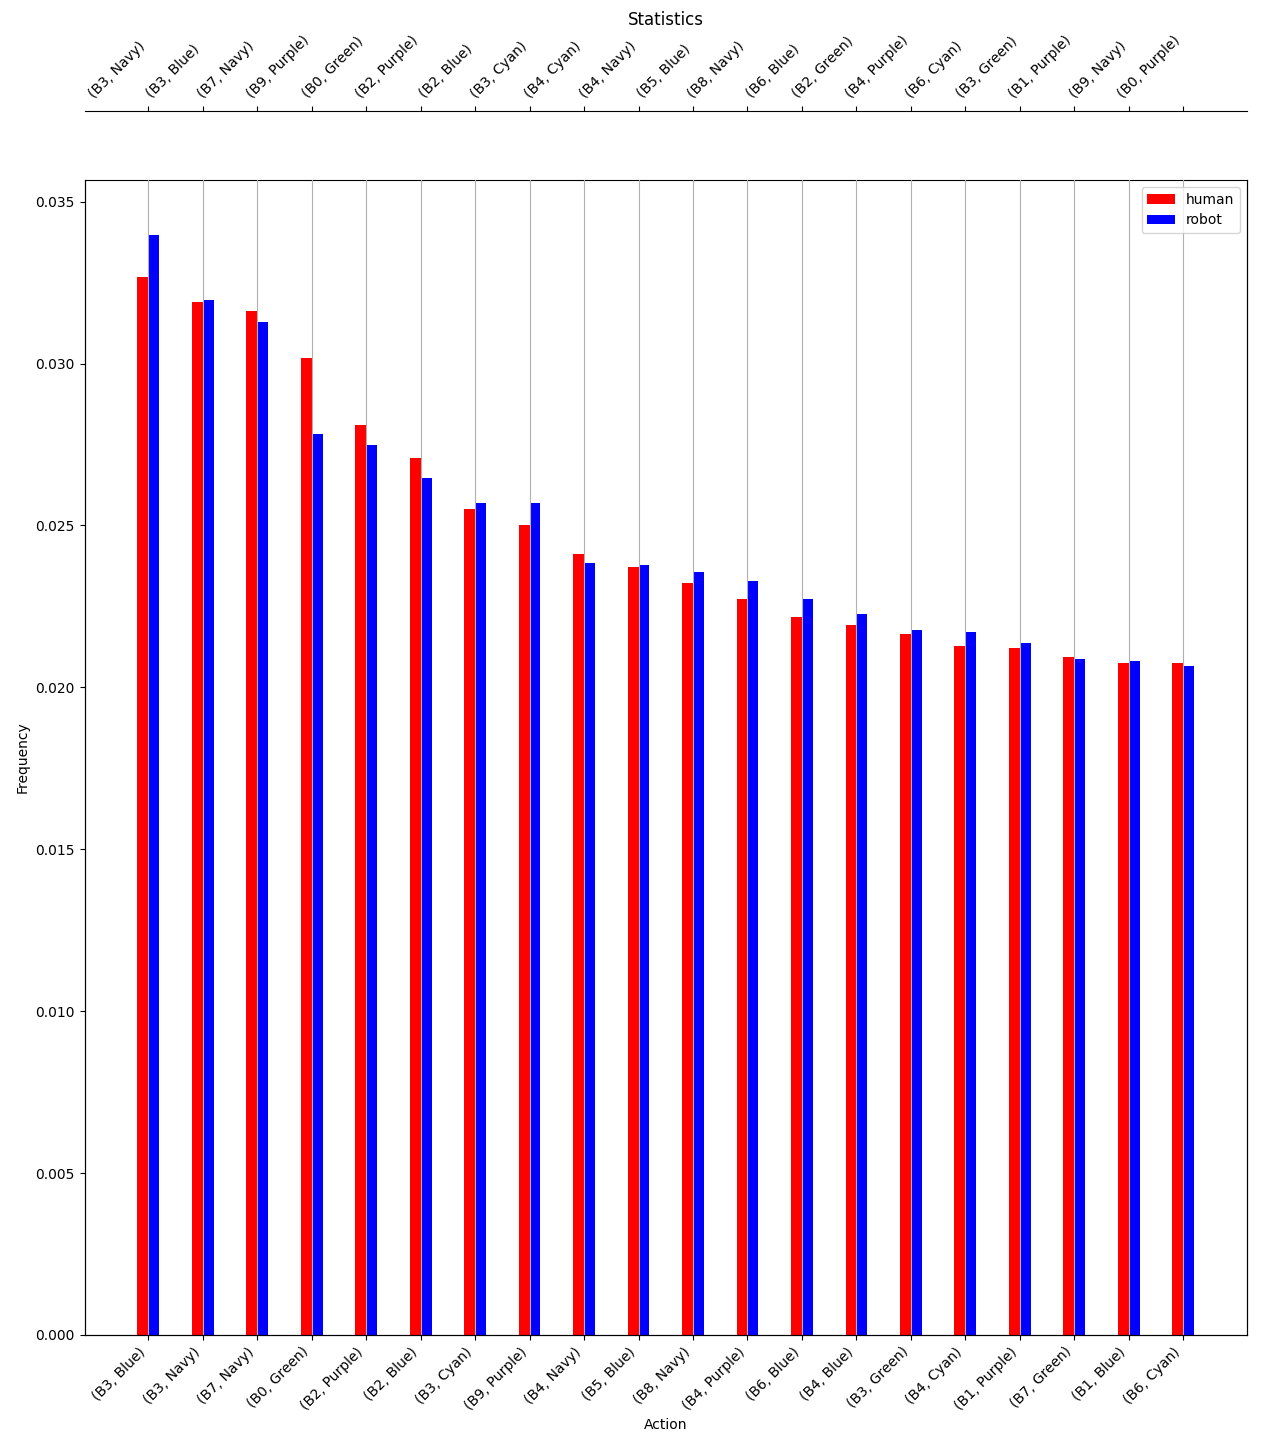
\includegraphics[width=\textwidth]{images/cc-stats.png}
                \caption{}
                \label{fig:cc-stats}
            \end{subfigure}
            \caption{Results from simulating the interactions between players C and C. The left image shows an example solution to the game (a), and the right image presents a statistical analysis of the most frequently selected actions (b).}
            \label{fig:cc-simulation}
        \end{figure}
        % 
        
        Other than that, both agents have been thoroughly trained in isolation, exploring a wide range of states and ultimately converging to stable policies. This allows them to respond effectively and optimally, even when paired with agents with conflicting styles of play. Therefore, even in the case of the most incompatible pairings, the number of mistakes remains minimal, and these mistakes are not due to inadequate exploration, but rather to the inherent conflicts in the agents’ preferences. 

    \end{flushleft}

    \subsubsection{Extracting the Empirical Payoff Matrix}

    \begin{flushleft}

        .....\\~\\

    \end{flushleft}

    \subsubsection{Evaluating and Ranking Joint Policies}

    \begin{flushleft}

        .....\\~\\

    \end{flushleft}

\end{flushleft}